\documentclass{article}
\usepackage[usenames,dvipsnames]{color}
\usepackage{hw}
\usepackage{bm}
\usepackage{amsmath}
\usepackage{graphicx}
\usepackage[colorlinks=true,urlcolor=blue]{hyperref}
\usepackage{geometry}
\geometry{margin=1in}
\usepackage{float}
\setlength{\marginparwidth}{2.15cm}
\usepackage{booktabs}
%\usepackage{enumitem}
\usepackage{epsfig}
\usepackage{setspace}
\usepackage{parskip}
\usepackage{bbm}
\usepackage[]{algorithm2e}
\usepackage{comment}
\usepackage{pdfpages}
\usepackage{physics}
\usepackage{ulem}
\usepackage{hyperref}
\usepackage{macro}
\usepackage{enumerate}
\usepackage{mcode}
\usepackage{soul}

\title{mlsp - hw3 - 2019}
\author{mahmoudi} % adapted from abelinoj
\date{October 2019}

\begin{document}

\begin{center}
  \centerline{\textsc{\LARGE Homework 3}}
  \vspace{0.5em}
  \centerline{\textsc{\Large NMF - Clustering - Sparse Optimization - SVMs}}
  \vspace{1em}
  \textsc{\large CMU 11-755/18-797: Machine Learning for Signal Processing (Fall 2020)} \\
  \vspace{1em}
  \centerline{OUT: October 23rd, 2020}
  \centerline{DUE: {\bf November 5th, 11:59 PM}}
\end{center}
\graphicspath{images}


\section*{START HERE: Instructions}


\begin{itemize*}

\item \textbf{Collaboration policy:} Collaboration on solving the homework is allowed, after you have thought about the problems on your own.  It is also OK to get clarification (but not solutions) from books or online resources, again after you have thought about the problems on your own.  There are two requirements: first, cite your collaborators fully and completely (e.g., ``Jane explained to me what is asked in Question 3.4'').  Second, write your solution {\em independently}: close the book and all of your notes, and send collaborators out of the room, so that the solution comes from you only.


\vspace{0.1in}
\item\textbf{Submitting your work:} Assignments should be submitted as PDFs using Canvas unless explicitly stated otherwise.  Please submit all results as ``report\underline{ }YourAndrewID.pdf'' in you submission.
\textbf{Each derivation/proof should be completed on a separate page}. Submissions can be handwritten, but should be labeled and clearly legible.  Else, submissions can be written in LaTeX.  Upon submission, label each question using the template provided by Canvas. Please refer to Piazza for detailed instruction for joining Canvas and submitting your homework.

\vspace{0.1in}
\item \textbf{Programming}: All programming portions of the assignments should be submitted to Canvas as well.  Please \texttt{zip} or \texttt{tar} all the code and output files together, and submit the compressed file together with the pdf report. We will not be using this for autograding, %but rather for plagiarism detection, 
meaning you may use any language which you like to submit.

\vspace{0.1in}
\item \textbf{Late submissions}: You are allowed 5 days of grace days \textbf{only} on homeworks. There is no restriction on how many late days you can use per homework. You don't need to inform the course staff if you use a late day.
\end{itemize*}

\newpage
\section{Understanding Boosting and ICA}


\subsection{Adaboost}

The figure below shows a data set that contains two classes ('+' and 'o'). The instances are labeled A-E.

\begin{center}
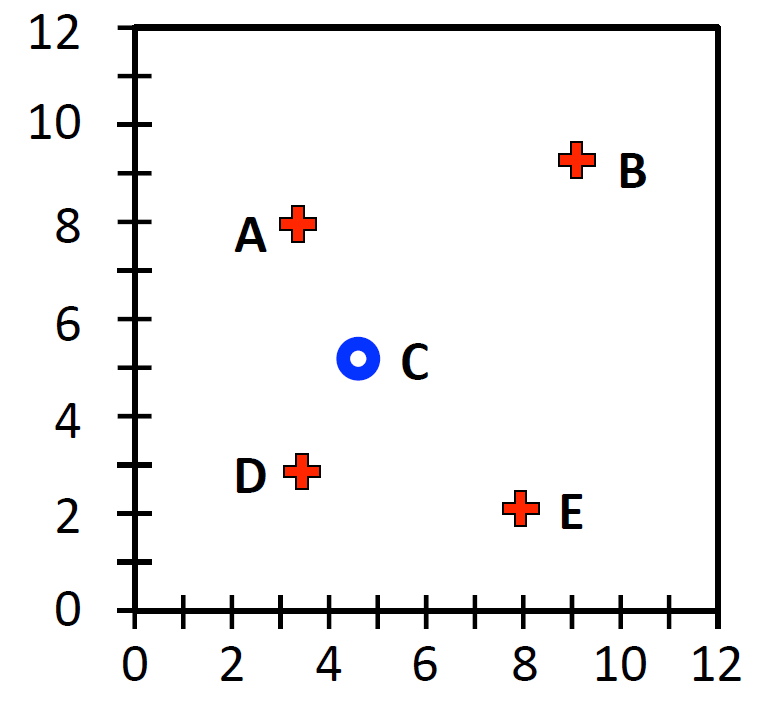
\includegraphics[trim={0cm 0 0 0},clip,scale=0.4]{figs/fig1.png}
\end{center}

If we train Adaboost to solve the classification problem.

\begin{enumerate}
    \item Which instances will have their weights increased at the end of the first boosting iteration? (Explain)
    \item What is the \textbf{minimum} number of iterations that the algorithm could take to achieve zero training error? (Explain)
    \item Is it possible to add another example to the data set to guarantee that boosting achieves zero training error in just two iterations? If so, how? If not, why?
\end{enumerate}

\subsection{Affine Transformation of Random variables}
Let ${\bf X}$ be a $d$-dimensional random vector with mean ${\bf \mu}$ and covariance matrix  $\Sigma$. Let ${\bf Y} = A{\bf X} + {\bf b}$, where $A$ is a $n \times d$ matrix and ${\bf b}$ is a $n$-dimensional vector.

\begin{enumerate}
    \item Show that the mean of ${\bf Y}$ is $A {\bf \mu } + {\bf b}$
    \item Show that the covariance matrix ${\bf Y}$ is $A \Sigma A^\top$
\end{enumerate}

\subsection{Difference between Correlation and Independence}

Consider the discrete random variable $X$ described as follows
$$ \mathbb{P}(X = i ) = \left\{ \begin{array}{ll} 1/3 & \text{ if } i = -1\\
1/3 & \text{ if } i = 0\\
1/3 & \text{ if } i = 1\end{array}\right.$$
We also define the random variable $Y = 1 - X^2$.

\begin{enumerate}
    \item Compute the values of $\mathbb{E}(X)$ and $\mathbb{E}(Y)$.
    \item Compute $\mathbb{E}(XY)$ and $Cov(X,Y)$. Are $X$ and $Y$ uncorrelated?
    \item Are $X$ and $Y$ independent? i.e., $\mathbb{P}(X = i\, , \, Y=j) = \mathbb{P}(X = i) \mathbb{P}(Y =j)$?
\end{enumerate}







\newpage
\section{Music Transcription}

\subsection{Projection}
 The song ``Polyushka Poly'' is played on the harmonica, the file name of the audio recording is  \texttt{\textbf{polyushka.wav}}, which can be found in the folder \texttt{\textbf{hw1materials}}. It has been downloaded from YouTube with permission from the artist.
\\
\\
A set of notes from a harmonica can be found in folder \texttt{\textbf{hw1materials/note15}}. You are required to transcribe the music. For transcription you must determine how each of the notes is played to compose the music.
\\
\\
You need to compute the spectrogram of the music file using your language/toolbox of choice, such as python (Librosa) or Matlab. First, read and load the audio file at 16000 Hz sample rate. 

% If you are using Matlab, you can use the following command:
% \begin{lstlisting}
% [s,fs] = audioread('filename');
% s = resample(s, 16000,fs);
% \end{lstlisting}

If you are using Python, you can use Librosa to load the wav file as follows (we also recommend using the \texttt{numpy} package for matrix operations below if you use python):

\begin{lstlisting}
import librosa
audio, sr = librosa.load(filename, sr = 16000)
\end{lstlisting}

Next, we can compute the complex Short-Time Fourier Transform (STFT) of the signal \textit{s} and its magnitude spectrogram. Use 2048 sample windows, which correspond to 64 ms analysis windows; overlap/hop length of 256 samples to 64 frames by second of signal. Different toolboxes should provide similar spectrograms. If you are using the Python Librosa library, you can use the following command:


% \begin{lstlisting}
% spectrogram = stft(s',2048,256,0,hann(2048));
% M = abs(spectrogram);
% phase = spectrogram./(M + eps);
% \end{lstlisting}

\begin{lstlisting}
spectrogram = librosa.stft(audio, n_fft=2048, hop_length=256, center=False, win_length=2048)
M = abs(spectrogram)
phase = spectrogram/(M + 2.2204e-16)
\end{lstlisting}

In this case, ${\bf M}$ represents the music file and should be a matrix of $1025 \times 8869$, where the rows correspond to the frequencies and the columns to time. A visualization (Librosa - specshow) of this matrix (spectrogram) should look like the following figure.
\begin{center}
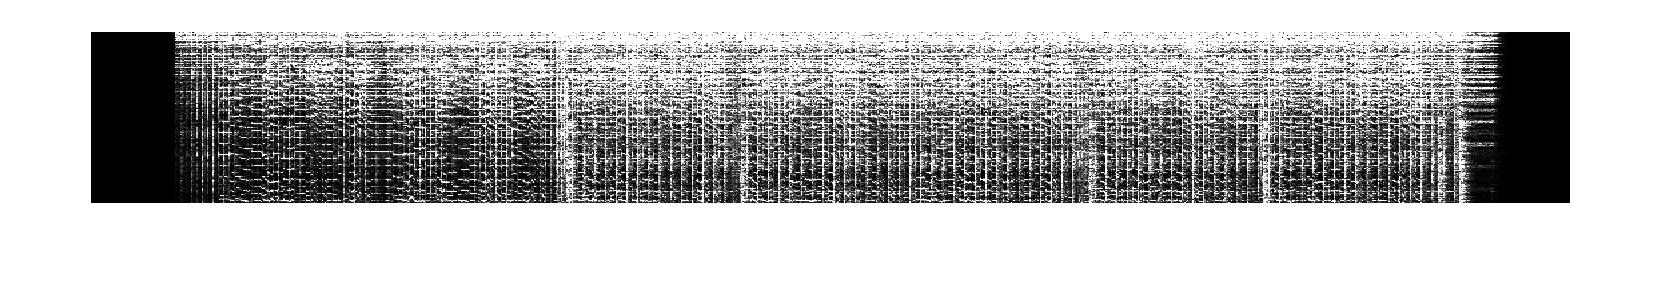
\includegraphics[trim={3cm 0 0 0},clip,scale=0.32]{figs/spectrogram.jpg}
\end{center}
To represent notes, you also need to compute the spectrogram of each note file. However, unlike the music file, we need to represent the matrix just as a one column vector. Hence, we can choose only one vector, or compute the mean of the matrix across time, etc. In this example, we select the middle column:
%[s, fs] = audioread('note_file');
%s = s(:,1);
%s = resample(s,16000,fs);
%spectrogram = stft(s', 2048, 256, 0, hann(2048));
% # find central frame
% middle = ceil(size(spectrogram,2)/2);
% note = abs(spectrogram(:,middle));
\begin{lstlisting}

# n is the spectrogram of the note 
import math
middle = n[:, int(math.ceil(n.shape[1]/2))]

\end{lstlisting}
To focus on the most relevant frequencies, we can clean up and normalize the note as follows:
\begin{lstlisting}
middle[middle < (max(middle)/100)] = 0
\end{lstlisting}

\newpage

% note(find(note < max(note(:))/100)) = 0;
Finally, you need to normalize this vector as follows,
% note = note/norm(note);
\begin{lstlisting}
middle = middle/np.linalg.norm(middle) # import numpy as np  
\end{lstlisting}


\begin{enumerate}
    \item Compute the joint contribution of all notes to the entire music. \\ 
    Mathematically, if $\mathbf{N} = [N_{1}, N_{2}, ...]$ is the note matrix where the individual columns are the notes, find the matrix $\mathbf{W}$ such that $\mathbf{N}\mathbf{W}\approx\mathbf{M}$, or that produce a small error $||\mathbf{M}-\mathbf{NW}||_{F}^{2}$. The $i_{th}$ row of $\mathbf{W}$ is the transcription of the  $i_{th}$ note. \underline{Submit the matrix ${\bf W}$ as  \texttt{problem1.csv} together with your code.}
    
    \item Recompose the music by ``playing'' each note according to the transcription you found in last question. \\ Set all negative elements in $W$ to zero and compute $\hat{M} = \mathbf{N}W$. \ul{Report the value of} $||\mathbf{M}-\hat{\mathbf{M}}||_{F}^{2} =  \sum_{i,j}(\mathbf{M}_{i,j}-\hat{\mathbf{M}}_{i,j})^{2}$ \ul{and submit the recomposed music named as \texttt{resythensized\_proj.wav} file.}
    
    To recover the signal from the reconstructed spectrogram $\hat{{\bf M}}$ we need to use the phase matrix we computed earlier from the original signal. Combine both and compute the Inverse-STFT to obtain a vector and then write them into a wav file. To compute the STFT and then write the wav file you can use the following python command:
    \begin{lstlisting}
    signal_hat = librosa.istft(M_hat*phase, hop_length=256, center=False, win_length=2048)
    librosa.output.write_wav("resynthensized_proj.wav", signal_hat, sr=16000)
    \end{lstlisting}
        % signal_hat = stft(np.dot(M_hat, phase), 2048, 256, 0, hann(2048))
    % audiowrite('wavfilename',signal_hat,16000)
\end{enumerate}


\subsection{Optimization and non-negative decomposition}

A projection of the music magnitude spectrogram (which are non-negative) onto a set of notes will result in negative weights for some notes. To explain this, let \textbf{M} be the (magnitude) spectrogram of the music, which is a matrix of size $D\times T$, where \textit{D} is the size of the Fourier Transform and \textit{T} is the number of spectral vectors in the signal. Let \textbf{N} be a matrix of notes of size $D\times K$, where \textit{K} is the number of notes and each column \textit{D} is the magnitude spectral vector of one note.

Conventional projection of \textbf{M} onto the notes \textbf{N} computes the following approximation:
$$\hat{\mathbf{M}} =\mathbf{N}\mathbf{W} $$
where $||\mathbf{M}-\hat{\mathbf{M}}||_{F}^{2} =  \sum_{i,j}(\mathbf{M}_{i,j}-\hat{\mathbf{M}_{i,j}})^{2}$ is minimized. Here, $||\mathbf{M}-\hat{\mathbf{M}}||_{F}$ is known as the Frobenius norm of $\mathbf{M} - \hat{\mathbf{M}}$, where $\mathbf{M}_{i,j}$ is the $(i,j)^{th}$ entry of \textbf{M} and $\hat{\mathbf{M}}_{i,j}$ is similarly the $(i,j)^{th}$ entry of $\hat{\textbf{M}}$. We will use later the definition of the Frobenius norm.
\\
\\
$\hat{\textbf{M}}$ is the projection of \textbf{M} onto \textbf{N}. Moreover, \textbf{W} is given by $\mathbf{W} = pinv(\mathbf{N})\mathbf{M}$ and \textbf{W} can be viewed as the transcription of \textbf{M} in terms of the notes in \textbf{N}. So, the $j^{th}$ column of $\mathbf{M}$, which we represent as $M_{j}$ is the spectrum in the $j^{th}$ frame of the music, which are approximated by the notes in \textbf{N} as follows:

$$\mathbf{M_{j}} = \sum_{i}\mathbf{N}_i\mathbf{W_{i,j}}$$
\\
where $\mathbf{N_i}$, the $i^{th}$ column of \textbf{N} represents the $i^{th}$ note and $\mathbf{W_{i,j}}$ is the (contribution) weight assigned to the $i^{th}$ note in composing the $j^{th}$ frame of the music.
\\
\\
The problem is that in this computation, we will frequently find $\mathbf{W}_{i,j}$ values to be negative. In other words, this model requires you to subtract some notes, since $\mathbf{W}_{i,j}\mathbf{N}_{i}$ will have negative entries.  Clearly, this is an unreasonable operation intuitively; when we actually play music, we never unplay a note (which is what playing a negative note would be).
%If $\mathbf{W}_{i,j}$ is negative, this is equivalent to subtracting note the weighted note $|\mathbf{W}_{i,j}|\mathbf{N}_{i}$ in the $j^{th}$ frame.
\\
\\
Also, $\mathbf{\hat{M}}$ may have negative entries due to the values in \textbf{W}. In other words, our projection of $\mathbf{M}$ onto the notes in $\mathbf{N}$ can result in negative spectral magnitudes in some frequencies at certain times. Again, this is meaningless physically -- spectral magnitudes cannot, by definition, be negative.
\\
\\
Hence, we will compute the approximation $\mathbf{\hat{M}=NW}$ with the constraint that the entities of $\mathbf{W}$ must always be greater than or equal to 0, \textit{i.e.} they must be non-negative. To do so we will use a simple gradient descent algorithm which minimizes the error $|| \mathbf{M - NW}|| ^2_F$, subject to the constraint that all entries in $\mathbf{W}$ are non-negative.

\begin{enumerate}

\item \textbf{Computing a Derivative}\\ \\
We define the following error function: \\
$$E = \frac{1}{DT} ||\mathbf{M-NW}||^2_F,$$
where $D$ is the number of dimensions (rows) in $\mathbf{M}$, and $T$ is the number of vectors (frames) in $\mathbf{M}$. \\
\\
\ul{Derive and write down the formula for $\frac{dE}{d\mathbf{W}}$.}
\\
\item \textbf{A Non-Negative Projection}\\ \\
We define the following gradient descent rule to estimate $\mathbf{W}$. It is an iterative estimate. Let $\mathbf{W}^0$ be the initial estimate of $\mathbf{W}$ and $\mathbf{W}^n$ the estimate after $n$ iterations. \\
We use the following project gradient update rule
$$
\hat{\mathbf{W}}^{n+1} = \mathbf{W}^n - \eta \frac{dE}{d\mathbf{W}} |_{\mathbf{W}^n}
$$
$$
\mathbf{W}^{n+1} = \max (\hat{\mathbf{W}}^{n+1},0)
$$
where $\frac{dE}{d\mathbf{W}}|_{\mathbf{W}^{n}}$ is the derivative of E with respect to $\mathbf{W}$ computed at $\mathbf{W} = \mathbf{W}^{n}$, and $max(\mathbf{\hat{W}}^{n+1},0)$ is a \textit{component-wise} flooring operation that sets all negative entries in $\mathbf{\hat{W}}^{n+1}$ to 0.
\\
\\
In effect, our \textit{feasible set} for values of $\mathbf{W}$ are $\mathbf{W}\succeq 0$, where the symbol $\succeq$ indicates that \textit{every} element of $\mathbf{W}$ must be greater than or equal to 0. The algorithm performs a conventional gradient descent update, and projects any solutions that fall outside the feasible set back onto the feasible set, through the \textit{max} operation.

Implement the above algorithm. Initialize $\mathbf{W}$ to a matrix of all 0s. Run the algorithm for $\eta$ values $(100,1000,10000,100000)$. Run 1000 iterations in each case. Plot E as a function of iteration number n for all $\eta$s in a figure. \ul{Show  this plot with some analysis in the separate page, and submit the best final matrix $\mathbf{W}$ (which resulted in the lowest error) named as \texttt{problem2W.csv} with the code.}

\item \textbf{Recreating the music}% (No points for this one)
\\
\\
For the best $\eta$ (which resulted in the lowest error) recreate the music using this transcription as $\mathbf{\hat{M}=NW}$. Resynthesize the music from $\hat{M}$. What does it sound like? \ul{Submit the resynthesized music named as \texttt{resynthesized\_nnproj.wav} with the code.}%You may return the resynthesized music to impress us (although we won't score you on it).

\end{enumerate}


\newpage



\section{Sparse recovery}

We have previously noted in class that given a dictionary $D$ and a data $X$ that can be composed as a \textit{sparse} combination of dictionary entries, i.e. we can write $X = D Y$, where $\|Y\|_0 \leq k$ for some small value of $k$, then $Y$ can be recovered from $X$ and $D$ using sparse recovery techniques. Specifically, we noted that this can be estimtated through the following minimization:

\begin{eqnarray}
\hat{Y} & = & \arg\min_Y \|X - DY\|_2^2 + \lambda \|Y\|_1
\end{eqnarray}

We will now see how this simple principle can be used to \textit{subsample} data and still recover it.  This principle is known as ``compressive sensing''.\\
\\
We will use an example to explain the concept. The example will also be your homework problem.

\subsection*{A little story: Cassini-Huygens}

The Cassini spacecraft was launched on 15 Oct 1997 and entered into orbit around Saturn on 1 July 2004.  Ever since it has been orbiting the ringed planet, taking thousands of pictures of Saturn, its rings, and its moons, and beaming them back to Earth. \href{https://saturn.jpl.nasa.gov/galleries/images/}{ Here} are some of the gorgeous pictures sent by Cassini to earth. Cassini is powered by about 33 kg of Plutonium-238, which will continue to provide power to the spacecraft until the end of its mission.
\\
\\
On Christmas day 2004 Cassini launched the Huygens probe towards Saturn's moon, Titan. Huygens landed on Titan on 14 Jan 2005. Unlike Cassini, Huygens was powered by a battery. By design, the module had no more than three hours of battery life, most of which was planned to be used during the descent onto Titan. Engineers expected to get at most only 30 minutes of data from the surface, much of which was in the form of pictures of Titan's surface and topography. \href{http://esamultimedia.esa.int/docs/titanraw/index.htm}{Here} are the incredible pictures sent by Huygens. 
\\
\\
Our ``story'' ends with this note: Huygens could only send 350 pictures before its batteries ran out of power. (An additional 350 pictures were lost because of a software bug due to which the channel they were sent on was ignored).

\subsection*{Compressive sensing to the rescue}
One of the main consumptions of on-board battery is for the \textit{transmission} of the pictures.  Each image must be adequately ``wrapped'' with error-correcting code and transmitted to the recipient (Huygens transmitted to both Cassini and the Earth). The amount of energy consumed to transmit a picture directly relates to the number of pixels captured -- more pixels require more energy both to capture and to transmit.
\\
\\
Let us now consider an alternate scheme.  

\begin{enumerate}
\item[(a)] \textit{\textbf{A note on image sparsity in the wavelet domain}}

It is well known that when considered in the wavelet transform domain, images are sparse. A wavelet transform can be viewed as a matrix operation (just as a discrete Fourier transform can). Let $I$ be any image (expressed as a vector). The wavelet transform $\mathcal{F}$ of the image can be computed as 
\begin{eqnarray}
\mathcal{F} & =& WI
\end{eqnarray}
where $W$ is the transform matrix. (In reality, the transform is viewed as a \textit{filterbank}, but we will assume the simpler model above for our discussion).

The image itself can be recovered from the transform as
\begin{eqnarray}
I & = & W^{-1} \mathcal{F}
\end{eqnarray}

For images, $\mathcal{F}$ is generally sparse, i.e. most of the components of $\mathcal{F}$ are zero or close to zero.\textbf{ We will use this to our benefit}.


\item[(b)] \textit{\textbf{Capturing \textit{one-pixel} masked integral images}}

Instead of simply snapping a picture directly, consider a scheme where Huygens would instead apply a \textit{random mask} to its camera and computes an \textit{integral} instead.  So, for instance, instead of capturing the entire image, Huygens applies a random mask to get the following picture
\begin{center}

\includegraphics[scale=0.4]{figs/saturnmask1.png}
\end{center}
and computes a \textbf{single} integral value
\begin{eqnarray}
P_1 &  = & \sum_{i,j} m_{i,j} I_{i,j}
\end{eqnarray}
where $m_{i,j}$ is the value of the mask at pixel $(i,j)$, and $I_{i,j}$ is the actual image value. Representing the mask as the vector $\mathbf{m}_1$, where the subscript $1$ is to indicate that this is the first such mask applied, Huygens' first measurement would be
\begin{eqnarray}
P_1 & = & \mathbf{m}_1^\top I
\end{eqnarray}

Similarly, applying a series of other such masks, e.g. 

\begin{center}

\includegraphics[scale=0.4]{figs/saturnmask2.png} $\qquad$ 
\includegraphics[scale=0.4]{figs/saturnmask3.png}
\end{center}

Huygens can now get a \textit{series of measurements} $P_1,~P_2,~P_3,\cdots,P_K$ of (scalar) measurements, where $P_i$ has been obtained using mask $\mathbf{m}_i$, and $K$ is the total number of measurements obtained in this manner. Representing all of the masks as a single matrix $\mathbf{M} = [\mathbf{m}_1~\mathbf{m}_2~\mathbf{m}_3\cdots\mathbf{m}_K]^\top$, and the measurements $P_i$ collectively as a vector $\mathbf{P} = [P_1~P_2~P_3\cdots P_K]^\top$, we can write
\begin{eqnarray}
\mathbf{P} & = & \mathbf{M}I
\end{eqnarray}

Note that $K$ may be far fewer than the number of pixels in the image. Huygens can now simply transmit $P_1 \cdots P_K$, and save on power. If $K < N$, where $N$ is the number of pixels in the image, Huygens could use the saved energy to take more pictures and transmit them. Since we are sending far fewer numbers than we would if we were to actually send the entire image, we will call these \textit{compressed} measurements.

\item[(c)] \textit{\textbf{Recovering the full image from the compressed measurements}}

But how then can the $N$-pixel pictures themselves be recovered from this sequence of $K$ compressed measurements?  For this we exploit the sparsity of images in the wavelet domain.  

Recall from our earlier discussion that we can represent $I = W^{-1} \mathcal{F}$, where $\mathcal{F}$ is sparse. Hence we can write
\begin{eqnarray}
\mathbf{P} & = & \mathbf{M}W^{-1}\mathcal{F}
\end{eqnarray}

Let $\mathbf{R} = \mathbf{M}W^{-1}$.  Remember that the random masks applied to the camera are \textit{known}, i.e. $\mathbf{M}$ is known. The inverse wavelet transform matrix $W^{-1}$ of course known.  Hence $\mathbf{R}$ is known. We can therefore write
\begin{eqnarray}
\mathbf{P} & = & \mathbf{R}\mathcal{F}
\end{eqnarray}
In other words, we are expressing the compressed measurements $\mathbf{P}$ as a sparse combination of the columns in a dictionary matrix $\mathbf{R}$.

To recover the image $I$ from the $K \times 1$ compressed measurement vector $\mathbf{P}$, it is sufficient to recover the $N \times 1$ sparse vector $\mathcal{F}$, since $I = W^{-1}\mathcal{F}$. We can do so using the sparse recovery technique we discussed in the context of dictionary-based representations, which we recalled above:
\begin{eqnarray}
\hat{\mathcal{F}} & = & \arg\min_{\mathcal{F}} \|\mathbf{P} - \mathbf{R}\mathcal{F}\|_2^2 + \lambda \|\mathcal{F}\|_1
\end{eqnarray}

The complete image can now be recovered as $I = W^{-1}\hat{\mathcal{F}}$. This is the basic concept behind compressive sensing.

We have managed to come up with a solution that enables Huygens to send far fewer numbers (only $K$) than the size of the image itself ($N$ pixels) and still recover the image. Huygens can now use the conserved battery to take more pictures.  We have thus rescued NASA's space exploration program!!

Having achieved these lofty goals, let us now return to a more mundane issue: homework problems.
\end{enumerate}


\subsection{$\ell_1$ minimization}

In this problem we give you compressed measurements from an image taken by Cassini (not Huygens).  We also give you the ``measurement matrix'' $\mathbf{R}$. You must recover the full image. (Note: we are referring to $\mathbf{R}$ in the above equations as the measurement matrix; more conventionally $\mathbf{M}$ would be called the measurement matrix).
\\
\\
You have been provided of the original image (\texttt{hw3material/problem3}). This is only for reference, to compute error; \textbf{we will not use it in recovery computations}. It is a $128 \times 128$ image with a total of 16384 pixels. Note that the sparse wavelet transform $\mathcal{F}$ of the image will also have 16384 components, although most of them will be very small or 0. 

In the directory \texttt{hw3materials/problem3/data} you also can find  three sets of compressed measurements \texttt{P1024.csv}, \texttt{P2048.csv} and \texttt{P4096.csv}, and their corresponding measurement matrices \texttt{R1024.csv},  \texttt{R2048.csv} and  \texttt{R4096.csv}.  In each case the numbers represent the  number of measurements. Thus \texttt{P1024.csv} contains a $1024 \times 1$ vector, representing 1024 one-pixel measurements, and \texttt{R1024.csv} is a $1024 \times 16384$ matrix that gives the linear transform from the 16384-component sparse transform $\mathcal{F}$ to the measurement vector in \texttt{P1024}. In the same directory you will also find the file named \texttt{S.csv}. This file is required by matlab for image reconstruction, and is not part of the actual recovery algorithm. 
\\
\\
You are required to use the sparse recovery procedure to recover $\mathcal{F}$ for each of these three measurements, and to reconstruct the image.


\begin{enumerate}
\item For each of the three measurements, solve 
\begin{eqnarray}
\hat{\mathcal{F}} & = & \arg\min_{\mathcal{F}} \|\mathbf{P} - \mathbf{R}\mathcal{F}\|_2^2 + \lambda \|\mathcal{F}\|_1
\end{eqnarray}

We recommend setting $\lambda = 100$, although you may also try other values. We included a matlab implementation of a least-squares $\ell_1$ (\texttt{l1\_ls.m}) solver
from Stephen Boyd (\texttt{hw3materials/problem3}). Note however that this is not the best algorithm; there are other better algorithms for $\ell_1$ minimization. The \href{http://sparselab.stanford.edu/}{Stanford sparselab} page has several nice solvers. You may try these; some of them should give you better results. 

If you are using Python, we would recommend to use Lasso from Sklearn. However, feel free to explore other solvers written in Python. 

For each of the three measurements, reconstruct the original image using the recovered $\mathcal{F}$. You can do so using matlab through the following commands:
\begin{lstlisting}
S = csvread('S.csv');
Irec = waverec2(F',S,'db1');
\end{lstlisting}

or if you are using Python, use the \texttt{F2Coeffs.py} in the handout code. 

Compute the error $E = \sum_{i,j} (I(i,j) - I_{rec}(i,j))^2$, where $I(i,j)$ and $I_{rec}(i,j)$ are the $(i,j)$th pixel value in the original and recovered image respectively.

\ul{You will be required to include your errors of three measurements and show the reconstructed image in your report (specify which solver and what parameters do you use), and submit your code.} Submissions that report lower error will obtain better scores for this problem, so it is in your benefit to explore.
\end{enumerate}


\subsection{Iterative Hard Thresholding}
In the previous part we solved the problem of sparse recovery as one of $\ell_1$ minimization.  We do so since it is well known that minimizing the $\ell_1$ norm also often minimizes the $\ell_0$ norm of the solution; however our actual objective in sparse recovery is to find a solution that has minimal $\ell_0$ norm, i.e. the smallest number of non-zero elements! Often, the optimal $\ell_1$ minimized solution will differ significantly (and can be significantly worse) than the optimal $\ell_0$ minimized solution.
\\
\\
In this part of the problem we will solve the alternate optimization problem:
\begin{eqnarray}
\hat{\mathcal{F}} & = & \arg\min_{\mathcal{F}} \|\mathbf{P} - \mathbf{R}\mathcal{F}\|_2^2~~~~{\rm such~that}~~\|\mathcal{F}\|_0 \leq K
\end{eqnarray}
where $K$ is the level of sparsity desired in $\mathcal{F}$. This is clearly an $\ell_0$ \textit{constrained} optimization problem. $\|\mathcal{F}\|_0 \leq K$ specifies a \textit{feasible set}, which is the set of all vectors that have no more than $K$ non-zero elements (note that this is a non-convex set). Recall from our lecture on optimization that we can use the method of projected gradients for this problem.
\\
\\
The gradient of $ \|\mathbf{P} - \mathbf{R}\mathcal{F}\|_2^2$ w.r.t $\mathcal{F}$ is given by
\begin{eqnarray}
\nabla_{\mathcal{F}}  \|\mathbf{P} - \mathbf{R}\mathcal{F}\|_2^2 & = & -\mathbf{R}^\top (\mathbf{P} - \mathbf{R}\mathcal{F})
\end{eqnarray}
Representing the $n^{\rm th}$ iterate in an iterative estimate of $\mathcal{F}$ by $\mathcal{F}^n$,  the projected gradient descent algorithm to estimate $\mathcal{F}$ would be given by
\begin{eqnarray}
\mathcal{F}_{unconstrained}^{n+1} & = & \mathcal{F}^n + \eta \mathbf{R}^\top (\mathbf{P} - \mathbf{R}\mathcal{F}^n) \\
\mathcal{F}^{n+1} &= & P_K(\mathcal{F}_{unconstrained}^{n+1})
\end{eqnarray}
where $\eta$ is a step size. The operator $P_K$ in the second step of the algorithm simply sets the $N-K$ smallest elements (in magnitude) of $\mathcal{F}_{unconstrained}^{n+1}$ to zero, forcing it to be a $K-sparse$ vector.
\\
\\
The second step in the above iteration is the ``projection'' step of the projected gradient algorithm.  It provably \textit{projects} $\mathcal{F}_{unconstrained}^{n+1}$ onto the feasible set for $\mathcal{F}$, namely the set of all $K$-sparse vectors.
\\
\\
The above iteration is guaranteed to converge under specific conditions on $\mathbf{R}$, $K$ and $\eta$. This is captured nicely in the following algorithm known as ``\textbf{Iterative Hard Thresholding}'' (IHT), proposed by Tom Blumensath.

\newpage

\begin{enumerate}
\item [] \textit{\textbf{Iterative Hard Thresholding}}

\textbf{As a first step}, the IHT algorithm assumes that the individual columns of the measurement matrix $\mathbf{R}$ are vectors of norm $\leq 1$. So, if this condition is not satisfied, multiply ${\bf R}$ by a scalar $\alpha$ such that the norm of the columns of $\alpha {\bf R}$ is less than 1. Note that it is NOT convenient that $\alpha$ is too small. Determine the largest value of $\alpha$ to reach the condition.

The IHT algorithm then performs iterations of the following computation:
\begin{enumerate}
\item [1.] Choose a maximum sparsity level $K$ for your solution.
\item [2.] Initialize $\mathcal{F}_{unconstrained}^{0} = 0$. (Alternately, you could set it to any random value).
\item [3.] Iterate:
\[
\mathcal{F}^{n+1} = P_K(\mathcal{F}^n + \mathbf{R}^\top (\mathbf{P} - \mathbf{R}\mathcal{F}^n))
\]
until the error $\|\mathbf{P} - \mathbf{R}\mathcal{F}\|_2^2$ converges, or the maximum number of iterations is achieved.
\item [4.] The final output is $\hat{\mathcal{F}} = \mathcal{F}_{conv}$, where $\mathcal{F}_{conv}$ is the final estimate derived from the previous step.
\end{enumerate}

\item [] What you need to do are as follows.
\begin{enumerate}
\item [i.] Implement the IHT algorithm. \ul{Include your IHT implementation to your code as a single file (iht.m or iht.py)}
\item [ii.] For each of the three measurements in the previous problem, find the estimate $\hat{\mathcal{F}}$ and reconstruct the original image using the recovered $\hat{\mathcal{F}}$, as you already did it. Compute the error $E = \sum_{i,j} (I(i,j) - I_{rec}(i,j))^2$, where $I(i,j)$ and $I_{rec}(i,j)$ are the $(i,j)$th pixel value in the original and recovered image respectively.  \ul{Include these errors, show the reconstructed images in your report, and submit your code}. 

\textbf{Note}: In this problem, use $K = round(max(\frac{M}{4},\frac{N}{10}))$, where $M$ is the number of measurements, and $N$ is the size of the image. Set the maximum number of iterations to 500.

\textbf{Note 2}: If you need to redefine the dictionary as $\alpha {\bf R}$, then, you will find $\mathcal{F}$ such that ${\bf P} \approx \alpha{\bf R} \mathcal{F}$. However, you need to find $\mathcal{F}$ such that  ${\bf P} \approx {\bf R} \mathcal{F}$ . 

\item [iii.] You should find that the IHT solution is considerably worse than the $\ell_1$ minimization result. Can you give any intuition as to why this is so? \ul{Include your analysis to your report.}
\end{enumerate}
\end{enumerate}

% \subsection*{Submission Instructions}
% \subsubsection*{Problem 1a}
% You are going to recover images for $3$ different measures of $P$ and $R$. In the \texttt{data} folder for Problem 1, you will find three folders $1639$, $2048$, $4096$. Each of these folders have three variable $P$, $R$ and $S$ which you need for solving the problem. 

% \begin{enumerate}
% \item Write a function \texttt{p1a\_getF(P, R, lambda)} which returns the recovered $\mathcal{F}$. It takes $P$, $R$ and $\lambda$ as inputs. 
% \item Write a main script \texttt{p1a\_Main.m}, which loads matrices, pass them to \texttt{p1\_getF()} function and then reconstruct the image using the recovered $\mathcal{F}$. Running this script should get the job done. Show the recovered image, compute errors and any other necessary thing.  
% \item In your report, report the reconstruction error.
% \item Submit the reconstructed image in \texttt{result} folder of problem 1. You should submit both an image file as well as the actual recovered image matrix, $Irec$. Name them as \texttt{I\_1639a.png} and \texttt{I\_1639a.mat} respectively. 
% \item The image recovery and reconstruction error needs to be done for all three measurements, 1639, 2048 and 4096. Name your recovered image file accordingly.
% \end{enumerate}

% \subsubsection*{Problem 1b}
% You are going to recover images for $3$ different measures of $P$ and $R$. In the \texttt{data} folder for Problem 1, you will find three folders $1639$, $2048$, $4096$. Each of these folders have three variable $P$, $R$ and $S$ which you need for solving the problem. 

% \begin{enumerate}
% \item Write a function \texttt{iht(P, R, K, niter )} which implements IHT algorithm. It takes as input $P$, $R$, $K$ (sparsity level), $n_{iter}$ = number of iterations as inputs.  
% \item Write a main script \texttt{p1b\_Main.m}, which does rest of the stuff, similar to \texttt{p1a\_Main.m}.  
% \item Use $n_{iter} = 200$. 
% \item In your report, report the reconstruction error for all 3 measurements. 
% \item Submit the recovered image for all three measurements in \texttt{result} folder of problem 1. Name your recovered image file properly, \texttt{I\_1639b.png} etc.  
% \end{enumerate}






\iffalse

\section{Source Separation using ICA}

%\subsection{Synthetic case}

In this problem, you have to implement your own version of ICA and apply it to source separation.\\
You are given 2 audio recordings, \texttt{sample1.wav} and \texttt{sample2.wav}. These can be found in the directory
\texttt{hw2materials/problem3.}

These recording were generated mixing two different audios. Your objective is to reconstruct the original sounds using ICA. Do the following steps:
\begin{enumerate}

    \item Implement your own version of ICA based on FOBI (Freeing Fourth Moments) method that we discussed in class. Write a function \texttt{ica} which receives as input a $2 \times N$ matrix and outputs a $2 \times N$ matrix where its rows are the extracted independent components. \ul{Submit your code}.
    
    \item Read the file \texttt{sample1.wav} and extract the audio signal \texttt{s1}. This should be a vector with 132,203 components. Read the file \texttt{sample2.wav} obtaining the signal \texttt{s2}. Both \texttt{s1} and \texttt{s2} have the same size. Transpose and concatenate these signals generating a matrix ${\bf M}$ with 2 rows and 132,203 columns.\\
    Apply the function \texttt{ica} on the matrix ${\bf M}$ and using the Matlab function \texttt{audiowrite}, save the components generated as \texttt{source1.wav} and \texttt{source2.wav} respectively. Don't forget ICA does not consider scale factors, so you may need to boost or decrease the resulting signal. \ul{Submit files \texttt{source1.wav} and \texttt{source2.wav}.}
    \item If ${\bf H}$ is a $2 \times N$ where its rows correspond to the output of \texttt{ica}, then we can consider that
    $$ {\bf M} = A {\bf H}$$
    In this case $A$ is the mixing matrix which produces our observation ${\bf M}$. Compute the $2 \times 2$ matrix for this case. \ul{Submit $A$ as \texttt{mixing\_matrix.csv}.} 
\end{enumerate}

\fi




%\newpage
%\section{Matlab Instructions}

\subsection{Computing the spectrogram}
Get the matlab file \verb|stft.m| in folder \texttt{\textbf{hw1materials}}.\\
\verb|stft.m| computes the complex spectrogram of a signal.\\
You can read a wav file into matlab as follows.
\begin{lstlisting}
[s,fs] = audioread('filename');
s = resample(s,16000,fs);
\end{lstlisting}

Above, we resample the signal to a standard sampling rate for convenience. Next, we can compute the complex short-time Fourier transform of the signal, and the magnitude spectrogram from it, as follows. Here we use 2048 sample windows, which correspond to 64ms analysis windows. Adjacent frames are shifted by 256 samples, so we get 64 frames/second of signal.

To compute the spectrogram of a recording, e.g. the music, perform the following.
\begin{lstlisting}
spectrum = stft(s',2048,256,0,hann(2048));
music = abs(spectrum);
sphase = spectrum./(abs(spectrum)+eps);
\end{lstlisting}
This will result in a 1025-dimensional (rows) spectrogram, with 64 frames(columns) per second of signal.
\\
\\
Note that we are also storing the phase of the original signal. We will need it later for reconstructing the signal. We explain how to do this later. The \textbf{eps} in this formula ensures that the denominator does not go to zero.
\\
\\
You can compute the spectra for the notes as follows. The following script reads the directory and computes spectra for all notes in it.
\begin{lstlisting}
notefolder = 'notes15/';
listname = dir([notesfolder '*.wav']);
notes = [ ];
for k = 1:length(listname)
    [s,fs] = audioread([notesfolder listname(k).name]);
    s = s(:,1);
    s = resample(s,16000,fs);
    spectrum = stft(s',2048,256,0,hann(2048));
    %Find the central frame
    middle = ceil(size(spectrum,2)/2);
    note = abs(spectrum(:,middle));
    %Clean up everything more than 40db below the peak
    note(find(note < max(note(:))/100)) = 0;
    note = note/norm(note);
    %normalize the note to unit length
    notes = [notes,note];
end
\end{lstlisting}
The ``\texttt{notes}'' matrix will have as many columns as there are notes (15 in our data). Each column represents a note. The notes will each be represented by a 1025 dimensional column vector.

\subsection{Reconstructing a signal from a spectrogram}

The recordings of the complete music can be read just as you read the notes. To convert it to a spectrogram, do the following. Let \textbf{reconstructedmagnitude} be the reconstructed magnitude spectrogram from which you want to compute a signal. In our homework we get many variants of this. To recover the signal we will use the \textbf{sphase} we computed earlier from the original signal.
\begin{lstlisting}
reconstructedsignal = stft(reconstructedmagnitude.*sphase,2048,256,0,hann(2048));
\end{lstlisting}





%==================================================================================================================================
%==================================================================================================================================
\newpage
\section{Submission Guide}

\subsection{Linear Algebra}
Please submit all results for this part in ``Report\underline{ }YourAndrewID.pdf'' in you submission
\subsection{Music Transcription Problem}
\textbf{2.1 Projection}\\
\\
The ``2.1'' subdirectory has a template file called Run\underline{ }problem21.m. Write your code into this script. There are instructions within the script on how to save your outputs. We repeat the instructions below.\\
\\
The scripts must be written so that we can simply run Run\underline{ }problem21.m from matlab within the directory, without any additional commands. If we cannot run the program, we cannot score you.\\
\\
1. Your solution will give you single ``score'' matrix $\mathbf{W}$. Save this as a single file named ``problem211.dat''
\\
\\
2. For this part, the synthesized music must be saved as ``problem212\underline{ }synthesis.wav'' within the ``results'' directory.\\
\\
\textbf{2.2 Optimization and non-negative decomposition}
\\
\\
1. For this part, return the solution in ``Report\underline{ }YourAndrewID.pdf'' in your submission.\\
\\
2. For this part, store the final $\mathbf{W}$ for each $\eta$ value in a text file called ``problem222\underline{ }eta\underline{ }xxx.dat'' where xxx is actual $\eta$ value. E.g. for $\eta = 0.01$, xxx will be ``0.01''. Plot the plot of $E$(total error) vs. iterations for each $\eta$ in a file called ``problem222\underline{ }eta\underline{ }xxx\underline{ }errorplot.png'', where xxx is the $\eta$ value. Also plot the $\eta$ vs. $E$ as a bar plot and save it in ``problem222\underline{ }eta\underline{ }vs\underline{ }E.png''.\\
\\
3. For this part, save the synthesized music in the ``results'' directory in a file called ``polyushaka\underline{ }syn.wav''\\
\\
\textbf{2.3 Linear Transformation}\\
\\
Your solution should include final magnitude spectrogram of audio D. Save this as a single file named ``problem23.mat''. Also save audio D as ``problem23\underline{ }audio.wav'' within the ``result'' directory. 

\end{document}
